%% Slides for ".NET Programming" by Chunyu Wang <chunyu@hit.edu.cn> %%

\section{文件和数据流}

\begin{frame}
\frametitle{数据流}
\begin{block}{\textit{Stream}}
  \CJKindent C\# 将 I/O 抽象成数据流的形式,屏蔽了不同 I/O 设备之间的差异,提
  供一致的面向流的行为方式,并通过抽象类 \texttt{Stream} 体现。
\end{block}
\begin{itemize}
\item 这些类都在 System.IO 命名空间中
\item 流的基本操作
\begin{itemize}
\item 从流读取:从流到数据结构的数据传输
\item 向流写入:从数据源到流的数据传输
\item 支持查找:对流内的当前位置进行的查询和修改
\end{itemize}
\end{itemize}
\end{frame}

\begin{frame}
\frametitle{Stream Architecture}
\centering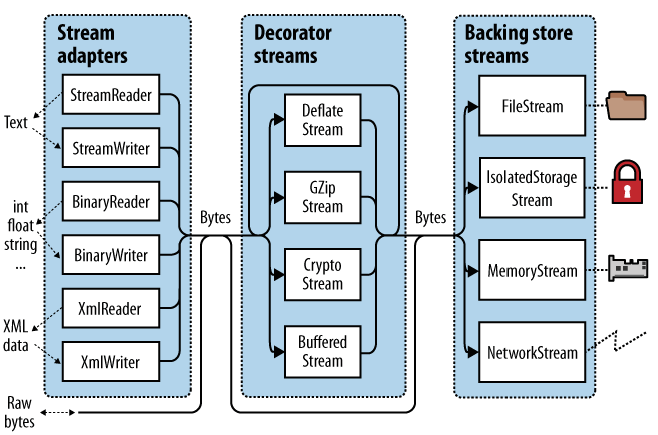
\includegraphics[width=11cm]{stream-arch}
\end{frame}


\begin{frame}
\frametitle{Stream 类}

抽象类 Stream 提供了对流的基本操作:
\begin{itemize}
\item void \textbf{Close}() --- 关闭数据流
\item void \textbf{Flush}() --- 将缓冲中的数据写入设备
\item int \textbf{ReadByte}() --- 读取一个用整数表示的字节
\item int \textbf{Read}(byte[] buf, int offset, int numBytes) \\
  将读入的字节写入 buf 缓冲中
\item long \textbf{Seek}(long offset, SeekOrigin origin)  \\
  在数据流中设置当前位置
\item void \textbf{WriteByte}(byte b) -- 向流中写入一个字节
\item void \textbf{Write}(byte[] buf, int offset, int numBytes) \\
  将 buf 中的数据写入流
\end{itemize}
\end{frame}

\begin{frame}
\frametitle{Stream 类的特性}
Stream 的派生类中,不一定都支持所有的操作,可如下判断:
\begin{itemize}
\item bool CanRead --- 是否可以读取
\item bool CanWrite --- 是否可以写入
\item bool CanSeek --- 是否支持定位
\item bool CanTimeout --- 是否会有超时
\item long Length --- 流的长度
\item long Position --- 目前在流中的位置,可以修改
\end{itemize}
\end{frame}


\begin{frame}<0| handout:0>
\frametitle{基本的I/O 字节流类}
\color{red}

Stream 是抽象类,如下几个是它的直接

\begin{tabular}[htbp]{l|l}
\hline
基本 I/O 流类 & 功能                                                     \\
\hline
BufferedStream & \small 用于给其他的流添加缓冲,提高性能                  \\
CryptoStream   & \small 在 System.Security.Cryptography 中,用于加密     \\
MemoryStream   & \small 在内存中直接访问所封装的数据                      \\
NetworkStream  & \small 在 System.Net.Sockets 中,用于封装网络连接上的流 \\
FileStream     & \small 基本的文件操作类                                  \\
\hline
\end{tabular}

\end{frame}

\begin{frame}
\frametitle{FileStream 类}
{\CJKindent FileStream 是对文件进行读取、写入和关闭操作,对管道、标准输入输出等设备的操作。}
\begin{figure}
  \centering
  %% Slides for ".NET Programming" by Chunyu Wang <chunyu@hit.edu.cn> %% -*- coding: utf-8 -*-

\begin{tikzpicture}[font=\footnotesize]
\tikzstyle{every node}=[anchor=west];
\node at (.3,4.7) {FileStream(file name, FileMode)};
\node at (.3,4.35) {FileStream(file name, FileMode, FileAccess)};
\node at (.3,4) {FileStream(file name, FileMode, FileAccess, FileShare)};
\draw (3.5,3.5) node (a1) {Append};
\draw (3.5,3.15) node (a2) {Create};
\draw (3.5,2.8) node (a3) {Open};
\draw (3.5,2.45) node (a4) {CreateNew};
\draw (3.5,2.1) node (a5) {OpenOrCreate};
\draw (3.5,1.75) node (a6) {Truncate};

\draw (5.1,3.5) node (b1) {Read};
\draw (5.1,3.15) node (b2) {\redwarn ReadWrite};
\draw (5.1,2.8) node (b3) {Write};

\draw (6.85,3.5) node (c1) {\redwarn None};
\draw (6.85,3.15) node (c2) {Read};
\draw (6.85,2.8) node (c3) {ReadWrite};
\draw (6.85,2.45) node (c4) {Write};

\foreach \x in {1,2,...,6}
\draw[thick] (3.4,3.8) |- (a\x);
\foreach \x in {1,2,3}
\draw[thick] (5,3.8) |- (b\x);
\foreach \x in {1,2,3,4}
\draw[thick] (6.75,3.8) |- (c\x);

\draw (.3,2.75) node {各个枚举量的成员};
\end{tikzpicture}

\end{figure}
\begin{itemize}
\item FileMode 指定文件的打开方式
\item FileAccess 指定文件的访问方式
\item FileShare 指定文件的共享方式
\end{itemize}
\end{frame}

\begin{frame}[fragile]
\frametitle{FileStream 示例}
\lstset{emph={WriteByte,ReadByte,Position,Length}}
\begin{lstlisting}
FileStream fs = new FileStream (@"C:\abc.txt", 
    FileMode.OpenOrCreate, FileAccess.ReadWrite);
byte[] data = new byte[5]{65,66,67,68,69}; // ABCDE

foreach (byte b in data){
  fs.WriteByte(b);}

fs.Position = 0; 

for (int i=0; i<fs.Length; i++)
  Console.Write((char) fs.ReadByte());

fs.Close();
\end{lstlisting}
\begin{itemize}
\item \texttt{fs.Position} 直接定位当前位置
\item \texttt{fs.Length} 直接取得文件长度
\end{itemize}
\end{frame}

\begin{frame}[fragile]
\frametitle{MemoryStream 类}
\CJKindent MemoryStream 主要用于临时数据存储,在内存中使用流的方式处理数据。
\begin{lstlisting}[escapeinside=<>]
// <使用> MemoryStream <缓冲一个文件>
FileStream fsIn = new FileStream(...);

MemoryStream ms = new MemoryStream();
int oneByte;

while ((oneByte = fsIn.ReadeByte()) != -1){
  ms.WriteByte ((byte)oneByte);
}
fsIn.Close();

// <流> ms <中的内容和文件一样,但效率更高>

\end{lstlisting}
\end{frame}

\begin{frame}[fragile]
\frametitle{BufferedStream 类}
\CJKindent BufferedStream 通过提供默认 4096 字节的缓冲,提高 I/O 的效率。这
几个 Stream 类都是基于字节的,即字节流 (\textit{Byte Stream})。
\begin{lstlisting}
Stream fs = new FileStream(@"C:\temp.txt"
    FileMode.OpenOrCreate, FileAccess.Write);

BufferedStream bs = new BufferedStream(fs);

byte[] data = new byte[5]{65,66,67,68,69}; // ABCDE

foreach (byte b in data){
  bs.WriteByte(b);}

bs.Close();
fs.Close();

\end{lstlisting}
\end{frame}

\begin{frame}
\frametitle{抽象类 TextReader/TextWriter}
\CJKindent 用于处理文本而不是原始字节的抽象类。
\medskip
\begin{itemize}
\setlength{\itemsep}{6pt plus 1pt}
\item TextReader 类
\begin{itemize}
\setlength{\itemsep}{4pt plus 1pt}
\item Peek(), Read(), ReadBlock(), ReadLine(), ReadToEnd()
\item Dispose(), Close()
\end{itemize}
\item TextWriter 类
\begin{itemize}
\setlength{\itemsep}{4pt plus 1pt}
\item Write(), WriteLine(), Flush(), Dispose()
\item Encoding, NewLine
\end{itemize}
\end{itemize}
\end{frame}

\begin{frame}[fragile]
\frametitle{StreamReader/StreamWriter}
\CJKindent 继承了 TextReader/TextWriter 用于处理流上的字符的类,即字符流
(\textit{Character Stream})。对于文件来说,处理基于 FileStream 的字符数据。
\medskip

多种构造函数,多种方式创建实例:
\lstset{emph={[4]path,s,append,e}}
\begin{lstlisting}
public StreamWriter(string path)
public StreamWriter(stream    s)

public StreamWriter(string path, bool append)
public StreamWriter(stream    s, bool append)

public StreamWriter(string path, bool append, Encoding e)
public StreamWriter(stream    s, bool append, Encoding e)
\end{lstlisting}
\end{frame}

\begin{frame}[fragile]
\frametitle{字符流示例}
\lstset{emph={Read,ReadToEnd}}
\begin{lstlisting}
FileStream fs = new FileStream(...); // Open a text file
StreamReader reader = new StreamReader(fs);

char[] buff = new char[4];
int count = reader.Read(buff,0,buff.Length);

string cup = reader.ReadToEnd();

fs.Position = 0;

string line = null;
while((line = reader.ReadLine() != null){
  Console.WriteLine(line);
}
\end{lstlisting}
\end{frame}

\begin{frame}[fragile]
\frametitle{编码转换的示例}
\begin{lstlisting}
using System; using System.IO; using System.Text;
public class Convert
{ static void Main()
  {
  StreamReader sr = new 
   StreamReader("G.txt",Encoding.GetEncoding("big5"));

  StreamWriter sw = new 
   StreamWriter("B.txt",false,Encoding.GetEncoding("gbk"));

  string str = null;
  
  while((str = sr.ReadLine()) != null)
  { sw.WriteLine (str); }

  sr.Close(); sw.Close();
  }
}
\end{lstlisting}
\end{frame}

\begin{frame}[fragile]
\frametitle{StringReader/StringWriter}
\CJKindent 通过 StringBuilder 存储的内存字符流,操作方式和流相同,但可以通过
GetStringBuilder 获取 StringBuilder 对象。

\begin{lstlisting}
StringWriter writer = new StringWriter();

writer.WriteLine("Hello world!");
writer.WriteLine("Some Text");

StringBuilder s = writer.GetStringBuilder();

s.Append("Some Other Text");
Console.WriteLine(s.ToString());

\end{lstlisting}
\end{frame}


\begin{frame}[fragile]
\frametitle{BinaryReader/BinaryWriter}
\CJKindent 用于处理值类型的数据的数据流,读写的数据使用计算机内部的二进制格式。

\begin{columns}[t]
  \column{.5\textwidth}
  \begin{itemize}
  \item BinaryWriter 重载各种数据的写操作\lstset{emph={[4]val}}
\begin{lstlisting}
void Write(byte   val)
void Write(sbyte  val)
void Write(int    val)
void Write(int[]  val)
void Write(double val)
void Write(char[] val)
void Write(string val)
...
\end{lstlisting}
  \end{itemize}
  \column{.5\textwidth}
  \begin{itemize}
  \item BinaryReader 提供不同读操作的方法
\begin{lstlisting}
bool   ReadBoolean()
byte   ReadByte()
sbyte  ReadSByte()
int    ReadInt32()
ulong  ReadUInt64()
double ReadDouble()
float  ReadSingle()
...
\end{lstlisting}
  \end{itemize}
\end{columns}
\end{frame}

\begin{frame}
\frametitle{Stream 之间的区别}
\begin{itemize}
\setlength{\itemsep}{6pt plus 1pt}
\item Stream 是流类型的抽象基类
\item TextReader/TextWriter 是处理字符(文本)的抽象基类
\item 基于字节的流类型:{\small FileStream, BufferedStream, MemoryStream}
\item 基于字符的流类型:{\small StreamReader/StreamWriter, StringReader/StringWriter}
\item 基于数据的流类型:{\small BinaryReader/BinaryWriter}
\end{itemize}
\begin{figure}
  \centering
  %% Slides for ".NET Programming" by Chunyu Wang <chunyu@hit.edu.cn> %%

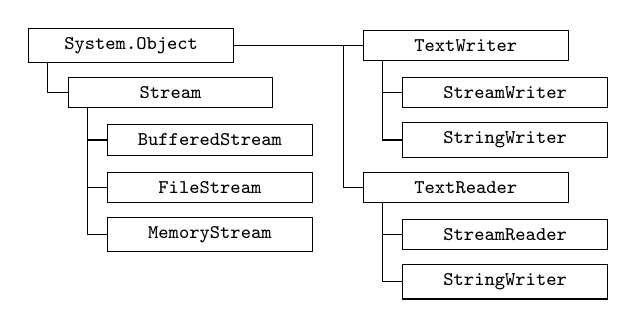
\begin{tikzpicture}
\tikzstyle{every node}=[anchor=west,draw,minimum width=2.6cm,fill=white,font=\ttfamily\scriptsize]
\node at (0,5) (a) {System.Object};
\node at (.5,4.4) (b) {Stream};
\node at (1,3.8) (b1) {BufferedStream};
\node at (1,3.2) (b2) {FileStream};
\node at (1,2.6) (b3) {MemoryStream};

\draw (a.south west) +(right:.25cm) |- (b);

\foreach \a in {b1,b2,b3}
\draw (b.south west) +(right:.25cm) |- (\a);

\node at (4.25,5)   (c) {TextWriter};
\node at (4.75,4.4)  (c1) {StreamWriter};
\node at (4.75,3.8)  (c2) {StringWriter};
\node at (4.25,3.2) (d) {TextReader};
\node at (4.75,2.6)  (d1) {StreamReader};
\node at (4.75,2)    (d2) {StringWriter};

\draw (c.south west) +(right:.25cm) |- (c1);
\draw (c.south west) +(right:.25cm) |- (c2);
\draw (d.south west) +(right:.25cm) |- (d1);
\draw (d.south west) +(right:.25cm) |- (d2);

\draw (a.east) -- (c.west);
\draw (c.west) +(left:.25cm) |- (d);

\end{tikzpicture}

\end{figure}
\end{frame}

\begin{frame}[fragile]
\frametitle{Console I/O}
\CJKindent Console I/O 定义在 System 命名空间中,提供基本的控制台操作。
\begin{itemize}
\item 标准 I/O 流 Console.In, Console.Out, Console.Error
\begin{lstlisting}
Console.In.ReadLine();   // TextReader
Console.Out.WriteLine(); // TextWriter
\end{lstlisting}
\item Console 类提供静态的方法,直接访问标准 I/O 流\\
Read(), ReadLine(), Write(), WriteLine()

\item static ConsoleKeyInfo \textbf{ReadKey}() \\
ConsoleKeyInfo 提供基本的按键信息,如所按的键值和 \texttt{ALT, CTRL, SHIFT} 等
\end{itemize}
\end{frame}

\begin{frame}
\frametitle{目录和文件}
\CJKindent System.IO 命名空间中还有用于操作文件和目录的类。
\begin{itemize}
\item DirectoryInfo 类,Directory 类
\begin{itemize}
\item Create(), Delete() --- 创建删除目录
\item GetDirectories(), GetFiles() --- 得到文件目录列表
\end{itemize}
\item FileInfo 类,File 类
\begin{itemize}
\item Open(), Create(), OpenWrite() --- 返回 FileStream 对象
\item OpenText(), CreateText() --- 返回 StreamWriter 对象
\end{itemize}
\item Path 类
\begin{itemize}
\item GetDirectoryName(), GetFullFileName() \dots
\end{itemize}
\end{itemize}
\end{frame}

\begin{frame}[fragile]
\frametitle{File 类}
静态类 File,使用绝对或相对文件名管理文件系统:
\begin{lstlisting}
bool Exists (string path); // true if present

void Delete (string path);
void Copy (string src, string dst);
void Move (string src, string dst);
void Replace (string src, string dst, string bak);
\end{lstlisting}
除文件操作,也可以修改文件属性等:
\begin{lstlisting}
FileAttributes GetAttributes (string path);
void SetAttributes (string path, FileAttributes attr);

DateTime GetCreationTime (string path); 
DateTime GetLastAccessTime (string path);
DateTime GetLastWriteTime (string path);
void SetCreationTime (string path, DateTime t);
void SetLastAccessTime (string path, DateTime t);
void SetLastWriteTime (string path, DateTime t);
\end{lstlisting}
\end{frame}

\begin{frame}[fragile]
\frametitle{File 类}
直接读取文件内容:
\begin{lstlisting}
byte[]   ReadAllBytes(string path);
string[] ReadAllLines(string path, Encoding e);
string   ReadAllText (string path, Encoding e);
IEnumerable<string> ReadLines(string path, Encoding e);
\end{lstlisting}
直接向文件写入内容:
\begin{lstlisting}
void WriteAllbytes(string path, byte[] buf);
void WriteAllLines(string path, IEnumerable<str> c);
void WriteAllText (string path, string content)
\end{lstlisting}
\end{frame}

\begin{frame}[fragile]
\frametitle{File 类举例}

\begin{lstlisting}
string filePath = @"c:\temp\test.txt";

FileAttributes fa = File.GetAttributes (filePath);

if((fa & FileAttributes.ReadOnly) > 0)
{ 
  fa ^= FileAttributes.ReadOnly;
  File.SetAttributes (filePath, fa); 
}

File.Delete (filePath);
\end{lstlisting}
\end{frame}

\begin{frame}[fragile]
\frametitle{FileSystemWatcher 类}
\CJKindent FileSystemWatcher 类用于监视文件系统的变化,可以捕获文件的创建、修改、
删除等事件。

\begin{itemize}
\item 特性
\begin{lstlisting}
bool   EnableRaisingEvents;
bool   IncludeSubdirectories;
string Filter;
string Path;
NotifyFilters NotifyFilter;
\end{lstlisting}
\item 事件
\begin{lstlisting}
FileSystemEventHandler Changed;
FileSystemEventHandler Created;
FileSystemEventHandler Deleted;
RenamedEventHandler    Renamed;
\end{lstlisting}
\end{itemize}
\end{frame}


\begin{frame}[fragile]
\frametitle{FileSystemWatcher 类举例}
\begin{lstlisting}
static void Main(string[] args)
{
  var w = new FileSystemWatcher(@"d:\download","*.txt");
  w.Created += watcher;     w.Deleted += watcher;
  w.Renamed += (s, e) => 
    Console.WriteLine("renamed "+e.OldName+"->"+e.Name);

  w.IncludeSubdirectories = true;
  w.EnableRaisingEvents = true;
  Console.WriteLine("Now I'm watching...");
  Console.ReadLine();
}

static void watcher(object sender, FileSystemEventArgs e)
{
 Console.WriteLine("file "+e.ChangeType+": "+e.FullPath);
}
\end{lstlisting}
\end{frame}


\section{网络}

\begin{frame}
\frametitle{网络}
\begin{itemize}
\item System.Net: {\scriptsize WebClient, WebResquest/WebResponse, Dns, \ldots}
\item System.Net.Socket: {\scriptsize Socket, TcpListener, TcpClient, UdpClient, \ldots}
\item System.Net.Mail: {\scriptsize SmtpClient, Attachment, MailAddress}
\end{itemize}
\centering 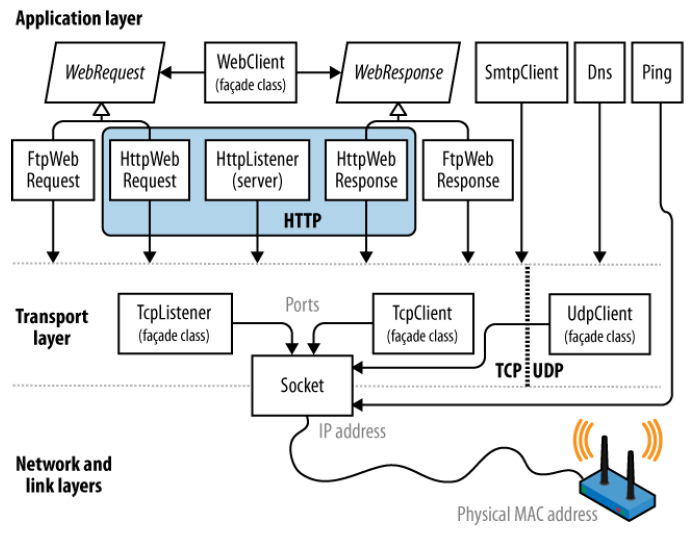
\includegraphics[width=7cm]{network-arch}
\end{frame}


\begin{frame}[fragile]
\frametitle{Web访问}
\begin{itemize}
\item WebRequest/WebResponse 类可以用来处理 HTTP 和 FTP 客户端访问
\item WebClient 实现了简单的 Web 客户端
\begin{lstlisting}
void DownloadFile(string url, string fileName);
string DownloadString(string url);
byte[] DownloadData (string url);
Stream OpenRead (string url);
byte[] UploadFile (string url, string fileName);
...
\end{lstlisting}
\item WebClient 示例
\begin{lstlisting}
WebClient c = new WebClient();
c.Proxy = null;
c.DownloadFile("http://localhost:8000/f.txt", "f2.txt");
System.Diagnostics.Process.Start("f2.txt");
\end{lstlisting}
\end{itemize}
\end{frame}


\begin{frame}[fragile]
\frametitle{Mail 和 SMTP}

\begin{itemize}
\item 邮件的使用 System.Net.Mail.SmtpClient
\end{itemize}
\begin{lstlisting}
SmtpClient client = new SmtpClient();
client.Host = "mail.myisp.net";
MailMessage mm = new MailMessage();

mm.Sender = new MailAddress ("kay@domain.com", "Kay");
mm.From   = new MailAddress ("kay@domain.com", "Kay");
mm.To.Add(  new MailAddress ("bob@domain.com", "Bob"));

mm.Subject  = "Hello!";
mm.Body     = "Hi there. Here's the photo!";
mm.IsBodyHtml = false;
mm.Priority = MailPriority.High;

Attachment a = new Attachment ("photo.jpg",
             System.Net.Mime.MediaTypeNames.Image.Jpeg);
mm.Attachments.Add (a);
client.Send (mm);
\end{lstlisting}
\end{frame}

\begin{frame}[fragile]
\frametitle{TCP 和 UDP}
\begin{itemize}
\item 客户端 TCP 直接使用 TcpClient 类,连接后得 Stream
\begin{lstlisting}[escapeinside=<>]
using(var client = new TcpClient (<address>, <port>))
using(NetworkStream n = client.GetStream())
{ // <Read and write to the network stream\ldots>
}
\end{lstlisting}
\item 服务端 TCP 直接使用 TcpListener 类
\item 通过 AcceptTcpClient 返回 TcpClient 对象
\begin{lstlisting}[escapeinside=<>]
TcpListener srv = new TcpListener (<address>, <port>);
srv.Start();

while(true)
  using(TcpClient c = listener.AcceptTcpClient())
  using(NetworkStream n = c.GetStream())
  { // <Read and write to the network stream\ldots>
  }
srv.Stop();
\end{lstlisting}
\end{itemize} 
\end{frame}

\begin{frame}[fragile]
\frametitle{多线程处理 TcpListener}
\begin{itemize}
\item 利用多线程同时处理多个 Client 
\lstset{emph={QueueUserWorkItem}}
\begin{lstlisting}[escapeinside=<>]
TcpListener t = new TcpListener(4343);
t.Start();

while (true) {
  TcpClient c = t.AcceptTcpClient();
  ThreadPool.QueueUserWorkItem(toClient, c);
}

private static void toClient(object o) {
    TcpClient c = (TcpClient)o;
    <$\cdots\cdots$>
}
\end{lstlisting}
\end{itemize}
\end{frame}

\begin{frame}[fragile]
\frametitle{单向 netcat 模拟}
\begin{itemize}
\item Server 写,Client 读
\begin{lstlisting}[escapeinside=<>]
// <Server's code, client use \texttt{netcat}>
TcpListener s = new TcpListener(4343);
s.Start();

using (TcpClient c = s.AcceptTcpClient())
using (NetworkStream n = c.GetStream())
{
  while (true)
  {
    string r = Console.ReadLine();
    byte[] buf = Encoding.GetEncoding(
                        "gb18030").GetBytes(r+"\n");
    n.Write(buf, 0, buf.Length);
  }
}
\end{lstlisting}
\end{itemize}
\end{frame}

\begin{frame}[fragile]
\frametitle{单向 netcat 模拟}
\begin{itemize}
\item Server 读,Client 写
\begin{lstlisting}[escapeinside=<>]
// <Server's code, client use \texttt{netcat}>
TcpListener s = new TcpListener(4343);
s.Start();

using (TcpClient c = s.AcceptTcpClient())
using (NetworkStream n = c.GetStream())
{
  while (true)
  {
    StreamReader sr = new StreamReader(n, 
                    Encoding.GetEncoding("gb18030"));
    string r = sr.ReadLine();
    Console.WriteLine(r);
  }
}
\end{lstlisting}
\end{itemize}
\end{frame}


% \begin{frame}[fragile]
% \frametitle{异步 IO}

% \begin{itemize}
% \item 在异步操作中完成 IO 操作
% \begin{lstlisting}
% public delegate void AsyncCallback(IAsyncResult ar);
% \end{lstlisting}
% \item Stream 的异步操作支持
% \begin{lstlisting}
% virtual IAsyncResult BeginRead(
%      byte[] buffer, int offset, int count, 
%           AsyncCallback callback, Object state );

% virtual int EndRead(IAsyncResult ar);
% \end{lstlisting}
% \begin{lstlisting}
% virtual IAsyncResult BeginWrite(
%      byte[] buffer, int offset, int count,
%           AsyncCallback callback, Object state );

% virtual void EndWrite(IAsyncResult ar);
% \end{lstlisting}
% \end{itemize}
% \end{frame}

\begin{frame}[fragile]
\frametitle{Network Stream 异步编程}
\begin{lstlisting}[escapeinside=<>]
NetworkStream n; byte[] buf; AsyncCallback callback;
void run()
{ buf   = new byte[8]; // <or 256, 1024 \ldots>
  callback += readFunc; 

  using(TcpClient client = new TcpClient(host, 4242))
  using(n = client.GetStream()){
    n.BeginRead(buf, 0, buf.Length, callback, null);
    while(true) { <\ldots\ for write \ldots\ >}
  }
}
static void readFunc(IAsyncResult r) {
  int len = n.EndRead(r);
  if (len > 0) {
    string s = Encoding.GetEncoding(
                       "gbk").GetString(buf, 0, len);
    Console.Write(s);
    n.BeginRead(buf, 0, buf.Length, callback, null);
  }
}
\end{lstlisting}
\end{frame}

\section{异步模型}

\begin{frame}
\frametitle{异步编程模型}
\begin{block}{\textit{Asynchronous Programming Model} (APM, 异步编程模型)}
\CJKindent  在主应用程序线程以外的线程中执行某个操作,但不阻塞主线程的继续执行。
\end{block}

\begin{itemize}
\item 同步:进程调用某方法后,需等待其结束,才能继续运行
\item 异步:进程调用某方法后,立即返回并继续运行,被调用方法在子线程中同时运行
\end{itemize}

\centering{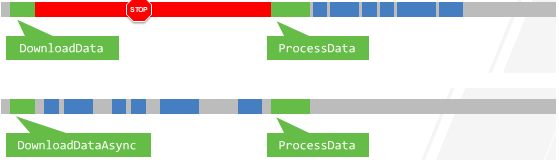
\includegraphics[scale=.6]{async-sync}}

\end{frame}


\begin{frame}[fragile]
\frametitle{基于 \textit{IAsyncResult} 的异步操作}

\begin{itemize}
\item \texttt{Callback} --- 异步回调
\begin{lstlisting}
delegate void AsyncCallback(IAsyncResult ar);
\end{lstlisting}
\item \texttt{IAsyncResult} --- 异步操作的中间过程
\begin{lstlisting}[escapeinside=<>]
public interface IAsyncResult {
  WaitHandle AsyncWaitHandle { get; } // <用于等待>
  Boolean    IsCompleted     { get; } // <用于轮询>
  Object     AsyncState      { get; } // <用于回调>
  Boolean    CompletedSynchronously { get; }
                                      // <基本不用>
}
\end{lstlisting}
\item \texttt{Begin\textbf{Xxx}} \ldots\ \texttt{End\textbf{Xxx}} --- 异步操作的开始和结束
\begin{lstlisting}[escapeinside=<>]
void Begin<\texttt{Xxx}>(<arg1>, <arg2>, <\ldots>, AsyncCallback, state);
TResult End<\texttt{Xxx}>(IAsyncResult);
\end{lstlisting}
\end{itemize}
\end{frame}


\begin{frame}[fragile]
\frametitle{委托的异步调用}

\begin{itemize}
\item 委托及方法
\begin{lstlisting}
delegate void Demo(int a, int b, int c);
\end{lstlisting}
\begin{lstlisting}
void func(int x, int y, int z) {
      Console.WriteLine("{0} {1} {2}", x, y, z);
}
\end{lstlisting}
\item 同步调用方法
\lstset{emph={Invoke}}
\begin{lstlisting}[escapeinside=<>]
Demo d = func;
d(1, 3, 5);         <// 同步调用>
d.Invoke(2, 4, 6);  <// 同步调用>
\end{lstlisting}
\item 异步调用方法
\lstset{emph={BeginInvoke}}
\begin{lstlisting}[escapeinside=<>]
Demo d = func;
IAsyncResult ar = d.BeginInvoke(1, 4, 7, null, null);
\end{lstlisting}
\end{itemize}
\end{frame}


\begin{frame}[fragile]
\frametitle{\emph{BeginInvoke} 与 \emph{EndInvoke}}
\begin{itemize}
\item 异步操作开始于 \textit{BeginInvoke} 方法
\begin{itemize}
\setlength{\itemsep}{4pt plus 1pt}
\item BeginInvoke 的参数随委托的参数而不同
\item BeginInvoke 的调用会立即返回,并返回 IAsyncResult 对象
\item BeginInvoke 发生异常,则不会执行委托
\item 委托会在线程池中执行
\end{itemize}
\item 可以有三种方式结束异步操作:等待、轮询和回调
\begin{itemize}
\setlength{\itemsep}{4pt plus 1pt}
\item 利用 IAsyncResult 和 EndInvoke 结束异步操作
\item EndInvoke 方法用于获取委托调用的结果
\item 如果异步操作未结束,EndInvoke 会阻塞直到结束
\item EndInvoke 必须使用对应的 IAsyncResult 对象作为参数
\item EndInvoke 参数还包括委托的 \textit{ref} 和 \textit{out} 参数
\end{itemize}
\end{itemize}

\end{frame}

\begin{frame}[fragile]
\frametitle{结束异步操作 --- 等待}

\begin{itemize}
\item 等待方式
\lstset{emph={BeginInvoke, EndInvoke}}
\begin{lstlisting}[escapeinside=<>]
static void longwork()  { <$\cdots$> }

  Action d = longwork;
  IAsyncResult ar = d.BeginInvoke(null, null);
  result = d.EndInvoke(ar);  // <主线程阻塞,等待完成>
\end{lstlisting}
或
\lstset{emph={BeginInvoke, WaitOne}}
\begin{lstlisting}[escapeinside=<>]
  IAsyncResult ar = d.BeginInvoke(null, null);
  WaitHandle w = ar.AsyncWaitHandle;
  w.WaitOne();               // <主线程阻塞,等待完成>
  result = d.EndInvoke(ar);  // <可选>
\end{lstlisting}
\end{itemize}
\end{frame}

\begin{frame}[fragile]
\frametitle{结束异步操作 --- 轮询}
\begin{itemize}
\item 轮询方式
\end{itemize}
\lstset{emph={IsCompleted, BeginInvoke}}
\begin{lstlisting}[escapeinside=<>]
public void longwork()  { <$\cdots$> }

  Action d = longwork;
  IAsyncResult ar = d.BeginInvoke(null, null);
  
  while(!ar.IsCompleted) {
     // <do something else>
  }
  result = d.EndInvoke(ar);
\end{lstlisting}
\end{frame}

\begin{frame}[fragile]
\frametitle{结束异步操作 --- 回调}

\begin{itemize}
\item 回调方式
\lstset{emph={callback, cbHandle}}
\begin{lstlisting}[escapeinside=<>]
public void longwork()  { <$\cdots$> }

public void Main(){
  Action d = longwork;
  AsyncCallback callback = cbHandle;
  IAsyncResult ar = d.BeginInvoke(callback, null);
  <$\cdots\ \cdots$>
}

public void cbHandle(IAsyncResult ar) {
  AsyncResult r = (AsyncResult) ar.AsyncDelegate;
  result = r.EndInvoke(ar);
}
\end{lstlisting}
\end{itemize}
\end{frame}

\begin{frame}
\frametitle{通用异步操作模型}

FCL中有很多支持 \textit{Begin}\texttt{Xxx}/\textit{End}\texttt{Xxx} 异步操作的类。

\begin{itemize}
\setlength{\itemsep}{6pt plus 1pt}
\item FileStream, NetworkStream
\begin{itemize}
\item[-] BeginRead / BeginWrite
\end{itemize}
\item TcpListener
\begin{itemize}
\item[-] BeginAcceptSocket / BeginAcceptTcpClient
\end{itemize}
\item HttpWebRequest
\begin{itemize}
\item[-] BeginGetRequestStream / BeginGetResponse
\end{itemize}
\item SqlCommand
\begin{itemize}
\item[-] BeginExecuteNonQuery
\item[-] BeginExecuteReader
\item[-] BeginExecuteXmlReader
\end{itemize}
\end{itemize}
\end{frame}

\begin{frame}[fragile]
\frametitle{回调方式举例(1)}

\begin{itemize}
\item myAction --- 异步用的委托类型
\item job --- 模拟长时间任务
\end{itemize}
\begin{lstlisting}
delegate int myAction (int i);

static int job(int n) {
    for (int i = 0; i < (int)n; i++) {
        Thread.Sleep( 100);
        Console.WriteLine(" *");
    }
    return Thread.CurrentThread.ManagedThreadId;
}
\end{lstlisting}
\end{frame}

\begin{frame}[fragile]
\frametitle{回调方式举例(2)}
\begin{itemize}
\item AsyncCallback --- 回调委托
\end{itemize}
\begin{lstlisting}
static void Main(string[] args)
{
    Console.WriteLine("Main Started...");
    myAction d = job;
    AsyncCallback callback = jobDoneHandle;

    IAsyncResult ar = d.BeginInvoke(10, callback, d);

    Console.WriteLine("Main Done.");
    Thread.Sleep(1500);
}
\end{lstlisting}
\end{frame}

\begin{frame}[fragile]
\frametitle{回调方式举例(3)}
\begin{lstlisting}
static void jobDoneHandle(IAsyncResult ar){
    // using System.Runtime.Remoting.Messaging;
    myAction d = (myAction)((AsyncResult)ar).AsyncDelegate;

    int id = d.EndInvoke(ar);
    Console.WriteLine("Thread ID: {0}", id);
}
\end{lstlisting}
\end{frame}


\section{串行化}

\begin{frame}
\frametitle{串行化}
\begin{block}{\textit{Serialization}}
\CJKindent 将对象或对象的集合转换为特定的格式,适于网络传递,存储在文件、数据
库内的过程,称为对象的串行化。

{\em 逆串行化} (\textit{Deserialization}) 过程正好相反,
将所存储的内容,转换回原来的对象。
\end{block}
.NET 支持三种主要的串行化:
\begin{itemize}
\item 二进制串行化,转换为二进制流(BinaryFormatter 类)
\item SOAP 串行化,转换为SOAP 标准格式(SoapFormatter 类)
\item XML 串行化,转换为XML 格式(XmlSerializer 类)
\end{itemize}
\end{frame}

\begin{frame}[fragile]
\frametitle{串行化的过程}
\begin{itemize}
\item 串行化时,根据对象的引用关系,构建一个对象图
\item 依次将该对象包括的全部成员对象串行化,完成深拷贝
\item 串行化发生前后会引发OnSerializing 和OnSerialized 事件
\item 串行化是基于对象的,因此不包括静态成员
\medskip \pause
\item 串行化通过不同Formatter 完成,有共同的接口IFormatter
\begin{lstlisting}
public interface IFormatter {
  object Deserialize(Stream s);
  void   Serialize(Stream s, object graph);
  // other members
}
\end{lstlisting}
\item 还提供了泛型接口 IGenericFormatter
\end{itemize}
\end{frame}

\begin{frame}[fragile]
\frametitle{二进制串行化}
\begin{itemize}
\item 使用 BinaryFormatter 
\item 定义在 System.Runtime.Serialization.Formatters.Binary
\end{itemize}
\begin{lstlisting}
  Circle c = new Circle();
  FileStream fstream = 
    new FileStream("data.out",FileMode.Create);
 
  BinaryFormatter bf = new BinaryFormatter();
  bf.Serialize(fstream,c);
  fstream.Close();
\end{lstlisting}
\end{frame}

\begin{frame}[fragile]
\frametitle{SOAP 串行化}
\begin{itemize}
\item 使用 SoapFormatter
\item 定义在 System.Runtime.Serialization.Formatters.Soap
\end{itemize}
\begin{lstlisting}
using System.Runtime.Serialization.Formatters.Soap;
[Serializable]
public class MyClass{
  public int a,b;
}
  MyClass obj = new MyClass();
  obj.a = 123;  obj.b = 456;
  IFormatter f = new SoapFormatter();
  Stream s =  new FileStream("data.xml",FileMode.Create);
  using (s) {
    f.Serialize(s , obj)
  }
\end{lstlisting}
\end{frame}

\begin{frame}[fragile]
\frametitle{可串行化属性}
\begin{itemize}
\item 串行化的类必须使用\texttt{[Serializable]} 属性
\item 不希望串行化的成员,需要用\texttt{[NonSerialized]} 属性
\item 可串行化属性无法通过继承得到
\end{itemize}
\begin{lstlisting}
[Serializable]
public class MyClass {
  public string str;
  public int i;

  [NonSerialized]
  int m;
}
\end{lstlisting}
\end{frame}

\begin{frame}[fragile]
\frametitle{不可串行化的成员}
\begin{itemize}
\item 未被串行化的成员,在逆串行化时,恢复为该类型的默认值
\item 但可以通过IDeserializationCallback 接口进行定制
\begin{lstlisting}
public interface IDeserializationCallback {
  void OnDeserialization(object sender);
}
\end{lstlisting}
\end{itemize}
\lstset{emph={[3]IDeserializationCallback,OnDeserialization}}
\begin{lstlisting}
[Serializable]
public class MyClass:IDeserializationCallback {
  [NonSerialized]
  IDbConnection m_Connection;
  ...
  public void OnDeserialization(object sender){
    m_Connection = new SqlConnection();
    m_Connection.ConnectionString = "...";
    m_Connection.Open();
  }
}
\end{lstlisting}
\end{frame}

\begin{frame}[fragile]
\frametitle{串行化和事件}
\begin{itemize}
\item 串行化事件:OnSerializing, OnSerialized
\item 逆串行化事件:OnDeSerializing, OnDeSerialized
\item 事件处理的方法,在被串行化的对象中实现
\item 事件的类型:
\begin{lstlisting}
void EVENTNAME(StreamingContext context);
\end{lstlisting}
\end{itemize}
\begin{lstlisting}
public class Chair {
  [OnDeserialized]
  void OnDeserialized(StreamingContext context) {
    if(Val == "abc") Val = "efg";
  }
}
\end{lstlisting}
\end{frame}

\begin{frame}[fragile]
\frametitle{串行化多个对象}
\begin{itemize}
\item 依次放入数据流进行串行化
\end{itemize}
\begin{lstlisting}
ClassA obj1 = new ClassA();
ClassB obj2 = new ClassB();

formatter.Serialize(stream, obj1);
formatter.Serialize(stream, obj2);

\end{lstlisting}
\begin{itemize}
\item 逆串行化,依次从数据流中读出即可
\end{itemize}
\begin{lstlisting}[escapeinside=<>]
// <\dots{} \dots{}>
ClassA a = (ClassA) formatter.Deserialize(stream);
ClassB b = (ClassB) formatter.Deserialize(stream);
\end{lstlisting}
\end{frame}

% Local Variables:
% mode: LaTeX
% TeX-master: "part-04.tex"
% TeX-header-end: "% End-of-Header$"
% TeX-trailer-start: "% Start-of-Trailer$"
% coding: utf-8
% End:
